\documentclass[letterpaper,twocolumn,12pt]{article}
\usepackage{usenix-2020-09}

% to be able to draw some self-contained figs
\usepackage{tikz}
\usepackage{amsmath}
\usepackage{hyperref}

% % inlined bib file
% \usepackage{filecontents}

% %-------------------------------------------------------------------------------
% \begin{filecontents}{\jobname.bib}
% %-------------------------------------------------------------------------------
% @Book{arpachiDusseau18:osbook,
%   author =       {Arpaci-Dusseau, Remzi H. and Arpaci-Dusseau Andrea C.},
%   title =        {Operating Systems: Three Easy Pieces},
%   publisher =    {Arpaci-Dusseau Books, LLC},
%   year =         2015,
%   edition =      {1.00},
%   note =         {\url{http://pages.cs.wisc.edu/~remzi/OSTEP/}}
% }
% @InProceedings{waldspurger02,
%   author =       {Waldspurger, Carl A.},
%   title =        {Memory resource management in {VMware ESX} server},
%   booktitle =    {USENIX Symposium on Operating System Design and
%                   Implementation (OSDI)},
%   year =         2002,
%   pages =        {181--194},
%   note =         {\url{https://www.usenix.org/legacy/event/osdi02/tech/waldspurger/waldspurger.pdf}}}
% \end{filecontents}

%-------------------------------------------------------------------------------
\begin{document}
%-------------------------------------------------------------------------------

%don't want date printed
\date{}

% make title bold and 14 pt font (Latex default is non-bold, 16 pt)
\title{\Large \bf Towards CANLay: An X-in-the-loop Virtual Testbench for In-Vehicle Security Testing with Real-time Network Performance Monitoring}

% %for single author (just remove % characters)
% \author{
% {\rm Jacob Jepson}\\
% Colorado State University
% \and
% {\rm Subhojeet Mukherjee}\\
% Colorado State University
% % copy the following lines to add more authors
% \and
% {\rm Jeremy Daily}\\
% Colorado State University
% } % end author

\maketitle

%-------------------------------------------------------------------------------
\begin{abstract}
%-------------------------------------------------------------------------------
Your abstract text goes here. Just a few facts. Whet our appetites.
Not more than 200 words, if possible, and preferably closer to 150.
\end{abstract}

% -------------- Plan ----


% --------------



\section{Introduction}
%-------------------------------------------------------------------------------
In recent years automotive security has been a much talked about topic of research. 
Researchers \cite{checkoway_comprehensive_2011} have shown that remote interfaces on modern passenger vehicles can be used to intrude into the in-vehicle network of embedded controllers, also referred to as Electronic Control Units (ECU). 
MHD vehicles expose similar interfaces that can be used to control/disrupt critical functions \cite{mukherjee_practical_2016,burakova_truck_2016} typically operated by ECUs using sensors and actuators. 
To evaluate the effectiveness of their approaches, researchers have traditionally experimented on real-vehicles or homegrown testbed setups that mimic real vehicles. 
While most households in the United States have at least one passenger car\footnote{\url{https://www.statista.com/statistics/551403/number-of-vehicles-per-household-in-the-united-states/}}, this is not the same for medium and heavy-duty (MHD) vehicles. 
Moreover, creating homegrown testbeds is both logistically and economically challenging. To that end, the need for a publicly accessible testbench is imminent.

% The first criteria to this type of testbed is accessibility the ease with each the testbench can be accessed. 
There are two important criteria that reseach in this area has established for this type of testbench. The first is fidelity, i.e. the ability of the setup to replicate a real-world in-vehicle networking infrastructure. The second is adapability i.e. the ability to be reconfigured to suit different needs. It may be difficult to maximixe the extent to which both these criteria is achieved. The most adaptible testbed is the one in which ECUs as well as the network  configuration can be programmed on the fly. Existing solutions have enabled ECU virtualization but not network virtualization for real-world ECUs. In those setups, ECUs from different physical locations cannot be used in the same testbed, neither can networks be configured on demand, unless the ECU is virtualized.
We believe that having real-world ECUs in the testing setup is critical. This not only provides greater fidelity but also alleviates any concerns with intellectual privacy and availability on the ECUs. Another aspect to fidelity and adaptibility is the realization of vehicular conquality of the network 
Existing solutions 

In this 

% The problem of remotely accessible testbeds for automotive control systems has been addressed in the past \cite{tagarev_automotive_2021}. A recent survey on the same identified an issue with the adaptability, i.e. the ability to adapt to user demanded configurations. Of the testbeds covered in \cite{tagarev_automotive_2021} and the only effective solution is a portable hardware testbench, PASTA \cite{}. There are two ways to adaptibility, virtualizing the ECU and/or virtaulizeing the network configuration. Most existing solutions have suggested virtualizing the ECU by reprograming the hardware to user demands. While this is viable solution, To achieve both, existing techniques have used a full virtualization scheme. 

\section{Design Goals}
\begin{figure}[t!]
    \centering
    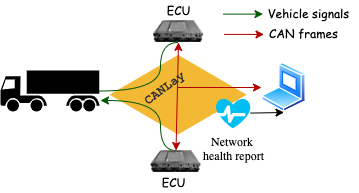
\includegraphics[width=\linewidth]{images/design_goal.drawio.png}
    \caption{Design Goal of CANLay}
    \label{fig:goal}
\end{figure}
% The overarching design goal of this project is eludiated through figure \ref{fig:goal}. In summary, our goal is to create an overlay over TCP/IP that can transport CAN frames and vehicle control signals to ECUs located in different subnets accross the globe. The control signals can be obtained from and fed back into a vehicle simulator that is the under the user's control. 
% The simulator is expoted to be useful in controlling the sensory inputs to the ECUs as well realize the effect of actuation. The overlay is expected to serve two purposes: create user demanded network configurations and make use of ECUs from different physical locations, possibly crowsourced. This model is designed in light of the software defined truck paradigm introduced in \cite{mukherjee_towards_2021}. In pursuit of the above mentinoned design goals, we identified four tasks. These task, along with the associated challenges, are described next. 

% \paragraph{Overlay Connection Management}
% \paragraph{Facilitation of CAN Data Manipulation via Vehicle Control}
% \paragraph{Facilitation of Vehicle Control via CAN Data Manipulation}
% \paragraph{Enabling Crowdsourcing of ECUs}



\section{Design}
\begin{figure*}[t!]
    \centering
    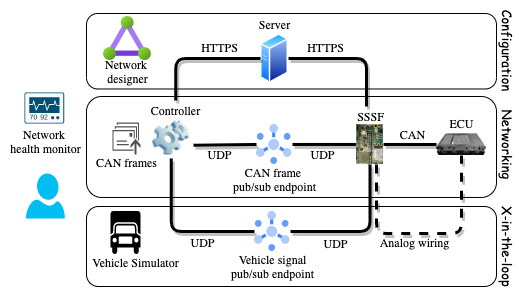
\includegraphics[width=\linewidth]{images/system_design.drawio.png}
    \caption{Proposed System}
    \label{fig:goal}
\end{figure*}

\subsection{Current Status of Development}

\subsection{Component Descriptions}
\subsubsection{Smart Sensor Simulator and Forwarder (SSSF)}
\subsubsection{Controller}
\subsubsection{Server}
\subsubsection{Vehicle Simulator}
\subsubsection{Publish/Subscribe Endpoints}
\subsubsection{User Interface to CAN}
\subsubsection{Network health monitor}

\subsection{Behavior Descriptions}
\begin{figure}[t!]
    \centering
    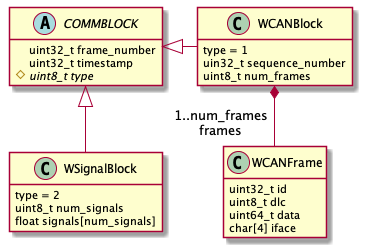
\includegraphics[width=\linewidth]{out/images/data_structures/data_structures.png}
    \caption{}
    \label{fig:}
\end{figure}

\subsubsection{Overlay Setup}
% \begin{figure}[t!]
%     \centering
%     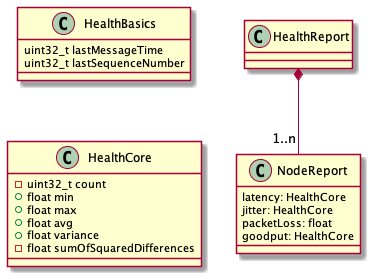
\includegraphics[width=\linewidth]{out/images/network_health/network_health.png}
%     \caption{}
%     \label{fig:}
% \end{figure}
\subsubsection{X-in-the-loop Simulation}
\begin{figure}[t!]
    \centering
    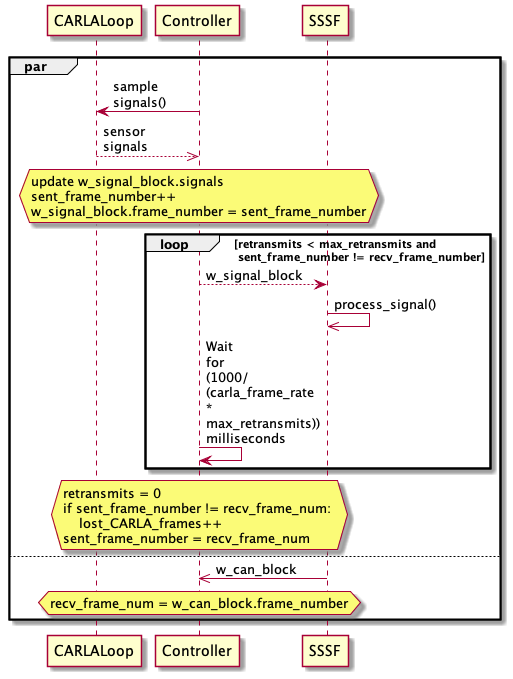
\includegraphics[width=\linewidth]{out/images/signal_control/signal_control.png}
    \caption{}
    \label{fig:}
\end{figure}
\subsubsection{CAN communication}
\begin{figure}[t!]
    \centering
    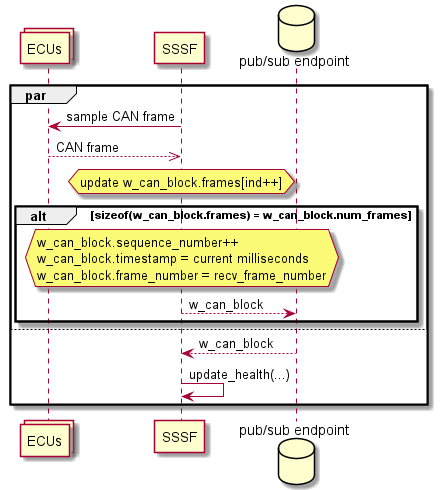
\includegraphics[width=\linewidth]{out/images/can_exchange/can_exchange.png}
    \caption{}
    \label{fig:}
\end{figure}
\subsubsection{Network health monitoring}
\begin{figure}[t!]
    \centering
    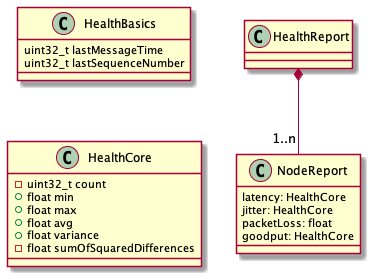
\includegraphics[width=\linewidth]{out/images/network_health/network_health.png}
    \caption{}
    \label{fig:}
\end{figure}
A health 

\section{Analysis}


%-------------------------------------------------------------------------------
\bibliographystyle{plain}
\bibliography{bib}

%%%%%%%%%%%%%%%%%%%%%%%%%%%%%%%%%%%%%%%%%%%%%%%%%%%%%%%%%%%%%%%%%%%%%%%%%%%%%%%%
\end{document}
%%%%%%%%%%%%%%%%%%%%%%%%%%%%%%%%%%%%%%%%%%%%%%%%%%%%%%%%%%%%%%%%%%%%%%%%
